
% Brent法のアニメーション
\begin{frame}{Brent法：ハイブリッド戦略の可視化}
  \begin{columns}
    \begin{column}{0.4\textwidth}
      \begin{itemize}
        \item \textbf{グレー領域}: 解を囲む区間 $[a, b]$
        \item \textcolor{blue}{\textbf{青丸}}: 現在の主要な3点 ($x, w, v$)
        \item \textcolor{red}{\textbf{赤丸}}: 今回の試行点 $u$
        \item \textcolor{green}{\textbf{緑破線}}: 採用された近似放物線
      \end{itemize}
      \vspace{1em}
      \small
      基本は放物線補間を試み、条件が悪い場合（緑線が出ない回）は安全な黄金分割を選択している様子がわかる。
    \end{column}
    \begin{column}{0.6\textwidth}
      \centering
      \only<1>{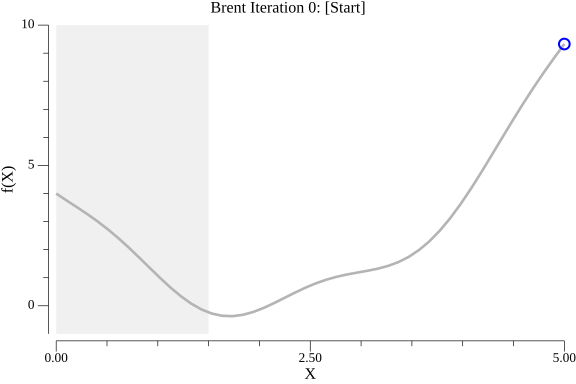
\includegraphics[width=\textwidth]{material/brent/output/brent_00.png}}
      \only<2>{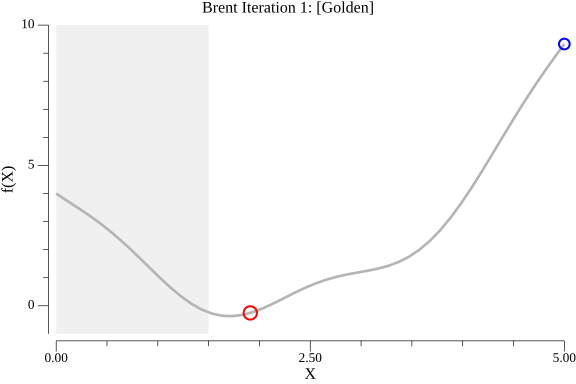
\includegraphics[width=\textwidth]{material/brent/output/brent_01.png}}
      \only<3>{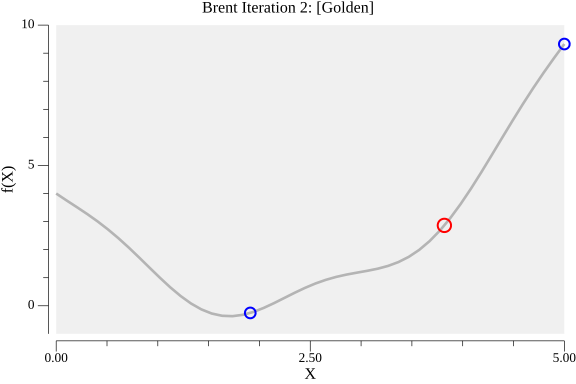
\includegraphics[width=\textwidth]{material/brent/output/brent_02.png}}
      \only<4>{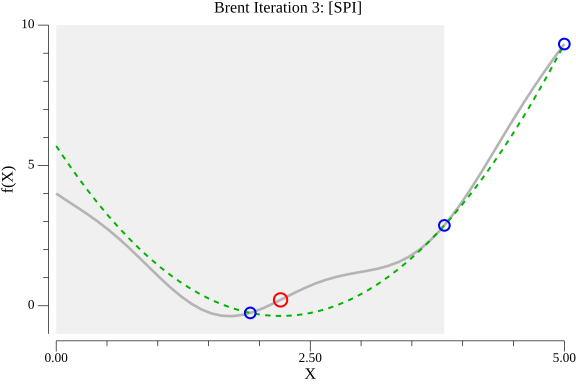
\includegraphics[width=\textwidth]{material/brent/output/brent_03.png}}
      \only<5>{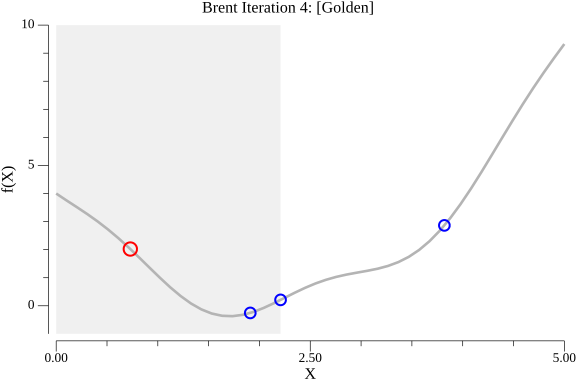
\includegraphics[width=\textwidth]{material/brent/output/brent_04.png}}
      \only<6>{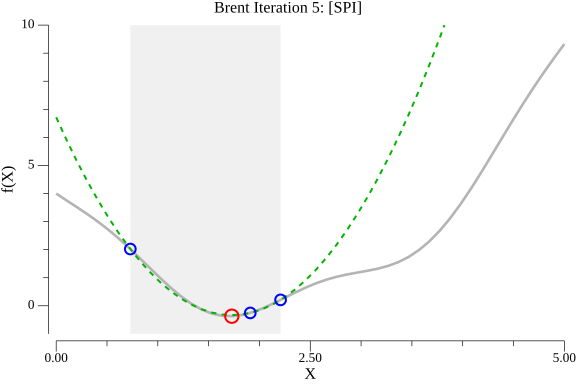
\includegraphics[width=\textwidth]{material/brent/output/brent_05.png}}
      \only<7>{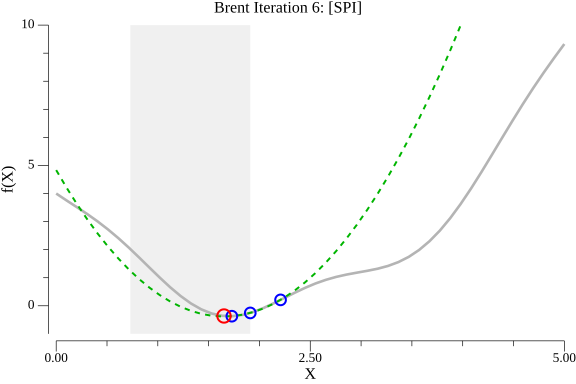
\includegraphics[width=\textwidth]{material/brent/output/brent_06.png}}
      \only<8>{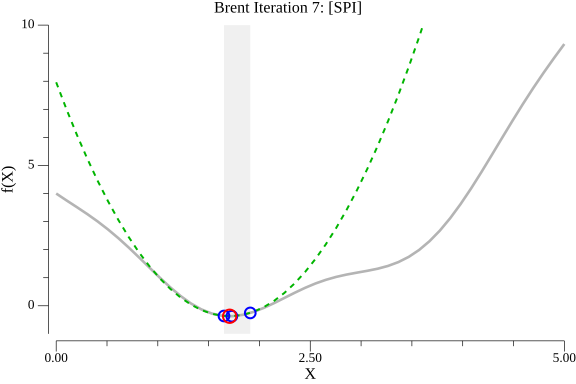
\includegraphics[width=\textwidth]{material/brent/output/brent_07.png}}
      \only<9>{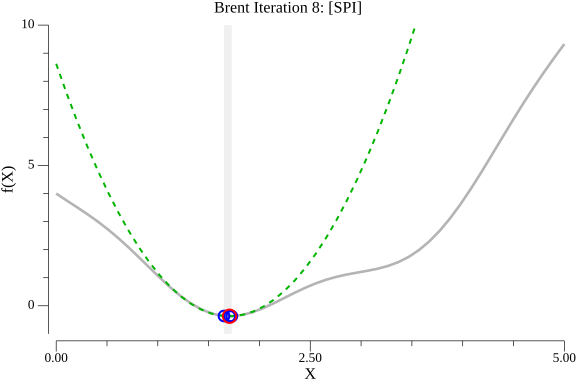
\includegraphics[width=\textwidth]{material/brent/output/brent_08.png}}
      \only<10>{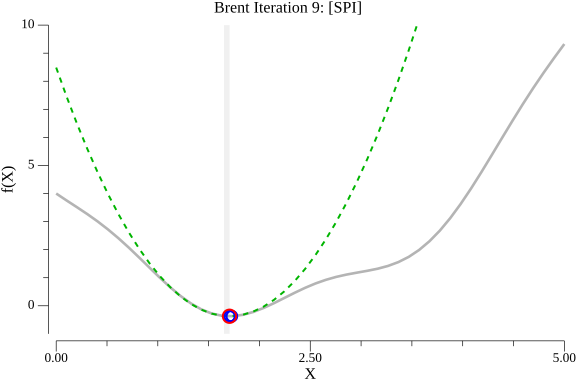
\includegraphics[width=\textwidth]{material/brent/output/brent_09.png}}
      \only<11>{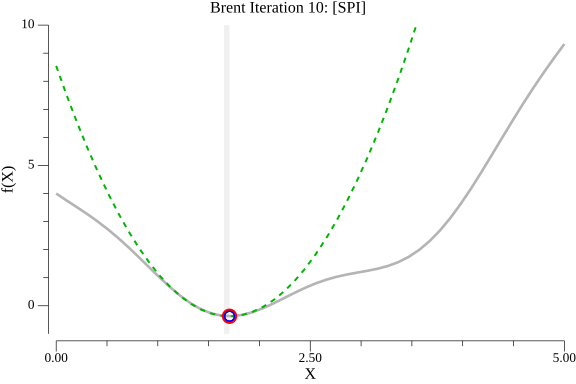
\includegraphics[width=\textwidth]{material/brent/output/brent_10.png}}
      \only<12>{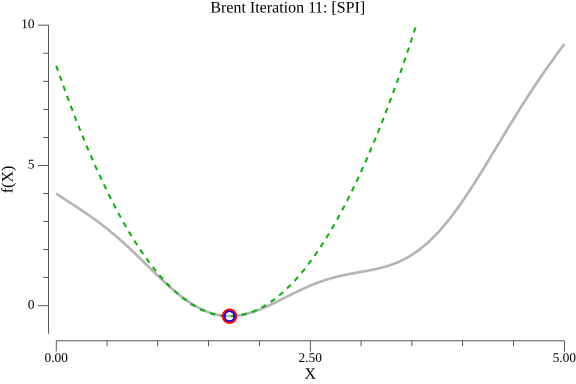
\includegraphics[width=\textwidth]{material/brent/output/brent_11.png}}
      \only<13>{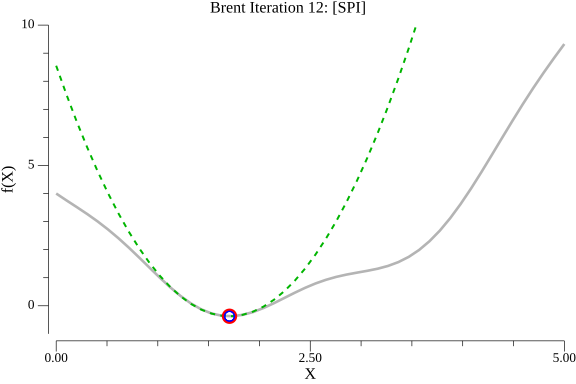
\includegraphics[width=\textwidth]{material/brent/output/brent_12.png}}
    \end{column}
  \end{columns}
\end{frame}
